
% \begin{table*}[h!]
%   \centering

%   % \renewcommand{\arraystretch}{1.15}
%   % \setlength{\tabcolsep}{6pt}
%   % \scriptsize     % CHAOQI: you can try this.
%   % \footnotesize
%   % \renewcommand{\arraystretch}{0.95}
%   % \setlength{\tabcolsep}{3pt}
%   \fontsize{7.4pt}{9pt}\selectfont
%   \renewcommand{\arraystretch}{0.98}
%   \setlength{\tabcolsep}{2pt}
  
%   % ---------------------- UP ----------------------
%   \subfloat{
%     \centering
%     \begin{tabular}{lc|c|ccc|cccc}
%       \toprule
%       Task & Metric &
%       DSP &
%       \makecell{Diffusion\\1X} &
%       \makecell{Diffusion\\2X} &
%       \makecell{Diffusion\\4X} &
%       \makecell{Diffusion +\\BSP 1X (ours)} &
%       \makecell{Diffusion +\\BSP 2X (ours)} &
%       \makecell{Diffusion +\\BSP 3X (ours)} &
%       \makecell{Diffusion +\\BSP 4X (ours)} \\
%       \midrule
%       \makecell{Cube \\ Picking} & \cellMetric &
%       \cellSRtime{18/20}{6.66s} &
%       \cellSRtime{19/20}{6.48s} &
%       \cellSRbold{20/20}{4.58s} &
%       \cellSRbold{20/20}{3.52s} &
%       \cellSRbold{20/20}{6.31s} &
%       \cellSRbold{20/20}{3.43s} &
%       \cellSRbold{20/20}{2.85s} &
%       \cellBothbold{20/20}{2.45s} \\
%       \midrule
%       \makecell{Table \\ Cleaning} & \cellMetric &
%       \cellSRtime{3/20}{49.47s} &
%       \cellSRtime{11/20}{41.40s} &
%       \cellSRbold{15/20}{28.87s} &
%       \cellSRtime{12/20}{23.31s} &
%       \cellSRbold{15/20}{36.97s} &
%       \cellSRtime{14/20}{20.81s} &
%       \cellTimebold{12/20}{17.30s} &
%       \cellSRtime{11/20}{18.05s} \\
%       \midrule
%       \makecell{Speed \\ Stacking} & \cellMetric &
%       \cellSRtime{3/20}{18.57s} &
%       \cellSRtime{14/20}{20.47s} &
%       \cellSRbold{15/20}{13.66s} &
%       \cellSRtime{9/20}{10.49s} &
%       \cellSRtime{14/20}{18.13s} &
%       \cellSRbold{15/20}{11.45s} &
%       \cellSRtime{11/20}{11.25s} &
%       \cellTimebold{7/20}{9.62s} \\
%       \bottomrule
%     \end{tabular}
%   }

%   \vspace{8pt}

%   % ---------------------- DOWN ----------------------
%   \subfloat{
%     \centering
%     \begin{tabular}{lc|c|ccc|cccc}
%       \toprule
%       Task & Metric &
%       DSP &
%       \makecell{Regression\\1X} &
%       \makecell{Regression\\2X} &
%       \makecell{Regression\\4X} &
%       \makecell{Regression +\\BSP 1X (ours)} &
%       \makecell{Regression +\\BSP 2X (ours)} &
%       \makecell{Regression +\\BSP 3X (ours)} &
%       \makecell{Regression +\\BSP 4X (ours)} \\
%       \midrule
%       \makecell{Cube \\ Picking} & \cellMetric &
%       \cellSRtime{18/20}{6.66s} &
%       \cellSRtime{18/20}{9.84s} &
%       \cellSRtime{15/20}{5.55s} &
%       \cellSRtime{19/20}{3.74s} &
%       \cellSRtime{19/20}{7.92s} &
%       \cellSRtime{19/20}{3.36s} &
%       \cellSRbold{20/20}{2.37s} &
%       \cellTimebold{19/20}{2.08s} \\
%       \midrule
%       \makecell{Table \\ Cleaning} & \cellMetric &
%       \cellSRtime{3/20}{49.47s} &
%       \cellSRtime{13/20}{49.70s} &
%       \cellSRtime{13/20}{34.48s} &
%       \cellSRtime{13/20}{23.57s} &
%       \cellSRbold{18/20}{38.47s} &
%       \cellSRbold{18/20}{19.11s} &
%       \cellSRtime{15/20}{13.34s} &
%       \cellTimebold{14/20}{11.80s} \\
%       \midrule
%       \makecell{Speed \\ Stacking} & \cellMetric &
%       \cellSRtime{3/20}{18.57s} &
%       \cellSRtime{8/20}{19.75s} &
%       \cellSRtime{4/20}{13.49s} &
%       \cellSRtime{8/20}{10.42s} &
%       \cellSRbold{16/20}{17.61s} &
%       \cellSRtime{13/20}{10.98s} &
%       \cellTimebold{7/20}{7.67s} &
%       \cellSRtime{0/20}{NA} \\
%       \bottomrule
%     \end{tabular}
%   }

% \caption{\todo \textbf{Real-world success rate and average completion time.}
% We report each method's success rate and average completion time on the real-world tasks. Completion time is averaged over successful trials only. For each task, we highlight the highest success rate and the shortest completion time. DSP denotes DemoSpeedup.}
% % \vspace{-20pt}
% \label{tab:act-dp-results}
% \end{table*}





% \begin{table*}[h!]
%   \centering

%   \fontsize{7.4pt}{9pt}\selectfont
%   \renewcommand{\arraystretch}{0.98}
%   \setlength{\tabcolsep}{2pt}
  
%   % ---------------------- UP ----------------------
%   \subfloat{
%     \centering
%     \begin{tabular}{lc|cc|cc|cc}
%       \toprule
%       Task & Metric &
%       \makecell{Diffusion\\1X} &
%       \makecell{Diffusion +\\BSP 1X (\textbf{ours})} &
%       \makecell{Diffusion\\2X} &
%       \makecell{Diffusion +\\BSP 2X (\textbf{ours})} &
%       \makecell{Diffusion\\4X} &
%       \makecell{Diffusion +\\BSP 4X (\textbf{ours})} \\
%       \midrule
%       \makecell{Cube \\ Picking} & \cellMetric &
%       \cellSRtime{19/20}{6.48s} &
%       \cellSRtime{\greenNum{20/20}}{\greenNum{6.31s}} &
%       \cellSRtime{20/20}{4.58s} &
%       \cellSRtime{\greenNum{20/20}}{\greenNum{3.43s}} &
%       \cellSRtime{20/20}{3.52s} &
%       \cellSRtime{\greenNum{20/20}}{\greenNum{2.45s}} \\
%       \midrule
%       \makecell{Table \\ Cleaning} & \cellMetric &
%       \cellSRtime{11/20}{41.40s} &
%       \cellSRtime{\greenNum{15/20}}{\greenNum{36.97s}} &
%       \cellSRtime{\greenNum{15/20}}{28.87s} &
%       \cellSRtime{14/20}{\greenNum{20.81s}} &
%       \cellSRtime{\greenNum{12/20}}{23.31s} &
%       \cellSRtime{11/20}{\greenNum{18.05s}} \\
%       \midrule
%       \makecell{Task 3} & \cellMetric &
%       \cellSRtime{x}{x} &
%       \cellSRtime{x}{x} &
%       \cellSRtime{x}{x} &
%       \cellSRtime{x}{x} &
%       \cellSRtime{x}{x} &
%       \cellSRtime{x}{x} \\
%       \midrule
%       \makecell{Task 4} & \cellMetric &
%       \cellSRtime{x}{x} &
%       \cellSRtime{x}{x} &
%       \cellSRtime{x}{x} &
%       \cellSRtime{x}{x} &
%       \cellSRtime{x}{x} &
%       \cellSRtime{x}{x} \\
%       \bottomrule
%     \end{tabular}
%   }

%   \vspace{8pt}

%   % ---------------------- DOWN ----------------------
%   \subfloat{
%     \centering
%     \begin{tabular}{lc|cc|cc|cc}
%       \toprule
%       Task & Metric &
%       \makecell{Regression\\1X} &
%       \makecell{Regression +\\BSP 1X (\textbf{ours})} &
%       \makecell{Regression\\2X} &
%       \makecell{Regression +\\BSP 2X (\textbf{ours})} &
%       \makecell{Regression\\4X} &
%       \makecell{Regression +\\BSP 4X (\textbf{ours})} \\
%       \midrule
%       \makecell{Cube \\ Picking} & \cellMetric &
%       \cellSRtime{18/20}{9.84s} &
%       \cellSRtime{\greenNum{19/20}}{\greenNum{7.92s}} &
%       \cellSRtime{15/20}{5.55s} &
%       \cellSRtime{\greenNum{19/20}}{\greenNum{3.36s}} &
%       \cellSRtime{19/20}{3.74s} &
%       \cellSRtime{\greenNum{19/20}}{\greenNum{2.08s}} \\
%       \midrule
%       \makecell{Table \\ Cleaning} & \cellMetric &
%       \cellSRtime{13/20}{49.70s} &
%       \cellSRtime{\greenNum{18/20}}{\greenNum{38.47s}} &
%       \cellSRtime{13/20}{34.48s} &
%       \cellSRtime{\greenNum{18/20}}{\greenNum{19.11s}} &
%       \cellSRtime{13/20}{23.57s} &
%       \cellSRtime{\greenNum{14/20}}{\greenNum{11.80s}} \\
%       \midrule
%       \makecell{Task 3} & \cellMetric &
%       \cellSRtime{x}{x} &
%       \cellSRtime{x}{x} &
%       \cellSRtime{x}{x} &
%       \cellSRtime{x}{x} &
%       \cellSRtime{x}{x} &
%       \cellSRtime{x}{x} \\
%       \midrule
%       \makecell{Task 4} & \cellMetric &
%       \cellSRtime{x}{x} &
%       \cellSRtime{x}{x} &
%       \cellSRtime{x}{x} &
%       \cellSRtime{x}{x} &
%       \cellSRtime{x}{x} &
%       \cellSRtime{x}{x} \\
%       \bottomrule
%       \end{tabular}
%   }


%   % ---------------------- UP ----------------------
%   \subfloat{
%     \centering
%     \begin{tabular}{lc|ccc}
%       \toprule
%       Task & Metric &
%       \makecell{DemoSpeedUp} &
%       \makecell{Diffusion +\\BSP 4X (\textbf{ours})} &
%       \makecell{Regression +\\BSP 4X (\textbf{ours})} \\
%       \midrule
%       \makecell{Cube \\ Picking} & \cellMetric &
%       \cellSRtime{18/20}{6.66s} &
%       \cellSRtime{\greenNum{20/20}}{2.45s} &
%       \cellSRtime{19/20}{\greenNum{2.08s}} \\
%       \midrule
%       \makecell{Table \\ Cleaning} & \cellMetric &
%       \cellSRtime{3/20}{49.47s} &
%       \cellSRtime{11/20}{18.05s} &
%       \cellSRtime{\greenNum{14/20}}{\greenNum{11.80s}} \\
%       \midrule
%       \makecell{Task 3} & \cellMetric &
%       \cellSRtime{x}{x} &
%       \cellSRtime{x}{x} &
%       \cellSRtime{x}{x} \\
%       \midrule
%       \makecell{Task 4} & \cellMetric &
%       \cellSRtime{x}{x} &
%       \cellSRtime{x}{x} &
%       \cellSRtime{x}{x} \\
%       \bottomrule
%     \end{tabular}
%   }

%   \vspace{8pt}

%   \caption{\textbf{Real-world success rate and average completion time.}
%   We report each method's success rate and average completion time on the real-world tasks.
%   Completion time is averaged over successful trials only.
%   For each task, we highlight the highest success rate and the shortest completion time.}
%   % \vspace{-20pt}
%   \label{tab:act-dp-results}
% \end{table*}





% \begin{figure*}[t]
%     \vspace{-20pt}

%     \centering
%     % \includegraphics[width=1\linewidth]{images/smoothness.pdf}
%     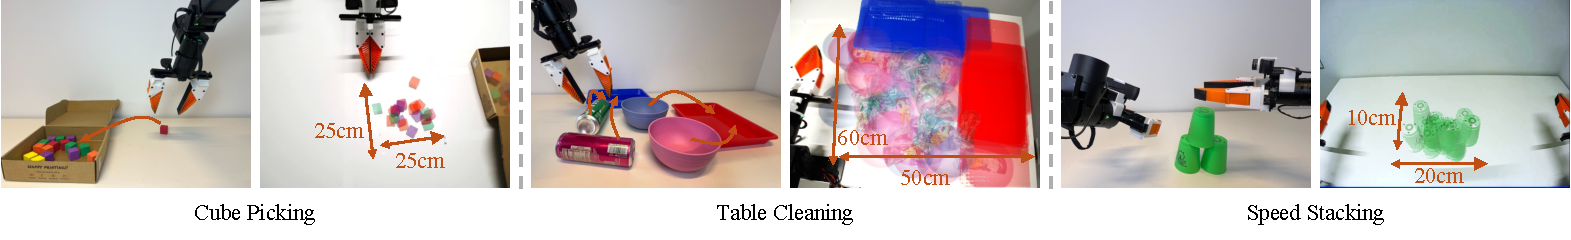
\includegraphics[width=1\linewidth]{images/real-world-task-setup.pdf}
%     \vspace{-15pt}
%     \caption{\textbf{Overview of the real-world tasks.} Task setups and corresponding object initialization distributions and workspace sizes for \pickcube, \cleantable, and \stackunstack.  These tasks vary in precision requirements, horizon length, and object interactions, highlighting the challenges of fast manipulation due to tight precision requirements, long task horizons, and complex object interactions.}
% \label{fig:real-world-setup}
% \vspace{-18pt}
% \end{figure*}


\begin{table*}[t]
  \centering
\vspace{-10pt}
    
  \fontsize{5.8pt}{6.8pt}\selectfont
  \renewcommand{\arraystretch}{0.92}
  \setlength{\tabcolsep}{1.2pt}

  \resizebox{\textwidth}{!}{
  \begin{tabular}{lc|cc|cc|cc||cc|cc|cc||ccc}
    \toprule
    Task & Metric
    & \multicolumn{6}{c||}{\textbf{Diffusion Policy}}
    & \multicolumn{6}{c||}{\textbf{Regression Policy}}
    & \multicolumn{3}{c}{\textbf{DemoSpeedUp Comparison}} \\
    \cmidrule(lr){3-8}
    \cmidrule(lr){9-14}
    \cmidrule(lr){15-17}

    & 
    & \multicolumn{2}{c|}{1X}
    & \multicolumn{2}{c|}{2X}
    & \multicolumn{2}{c||}{4X}
    & \multicolumn{2}{c|}{1X}
    & \multicolumn{2}{c|}{2X}
    & \multicolumn{2}{c||}{4X}
    & DemoSpeedUp
    & \makecell{Diff. +\\BSP 4X}
    & \makecell{Reg. +\\BSP 4X} \\
    \cmidrule(lr){3-4}
    \cmidrule(lr){5-6}
    \cmidrule(lr){7-8}
    \cmidrule(lr){9-10}
    \cmidrule(lr){11-12}
    \cmidrule(lr){13-14}

    & 
    & Diff.
    & \makecell{Diff. +\\BSP}
    & Diff.
    & \makecell{Diff. +\\BSP}
    & Diff.
    & \makecell{Diff. +\\BSP}
    & Reg.
    & \makecell{Reg. +\\BSP}
    & Reg.
    & \makecell{Reg. +\\BSP}
    & Reg.
    & \makecell{Reg. +\\BSP}
    & 
    & 
    & \\
    \midrule

    \makecell{Cube \\ Picking} & \cellMetric
    & \cellSRtime{19/20}{6.48s}
    & \cellSRtime{\greenNum{20/20}}{\purpleNum{6.31s}}
    & \cellSRtime{20/20}{4.58s}
    & \cellSRtime{\greenNum{20/20}}{\purpleNum{3.43s}}
    & \cellSRtime{20/20}{3.52s}
    & \cellSRtime{\greenNum{20/20}}{\purpleNum{2.45s}}
    & \cellSRtime{18/20}{9.84s}
    & \cellSRtime{\greenNum{19/20}}{\purpleNum{7.92s}}
    & \cellSRtime{15/20}{5.55s}
    & \cellSRtime{\greenNum{19/20}}{\purpleNum{3.36s}}
    & \cellSRtime{19/20}{3.74s}
    & \cellSRtime{\greenNum{19/20}}{\purpleNum{2.08s}}
    & \cellSRtime{18/20}{6.66s}
    & \cellSRtime{\greenNum{20/20}}{2.45s}
    & \cellSRtime{19/20}{\purpleNum{2.08s}} \\

    \midrule

    \makecell{Table \\ Cleaning} & \cellMetric
    & \cellSRtime{11/20}{41.40s}
    & \cellSRtime{\greenNum{15/20}}{\purpleNum{36.97s}}
    & \cellSRtime{\greenNum{15/20}}{28.87s}
    & \cellSRtime{14/20}{\purpleNum{20.81s}}
    & \cellSRtime{\greenNum{12/20}}{23.31s}
    & \cellSRtime{11/20}{\purpleNum{18.05s}}
    & \cellSRtime{13/20}{49.70s}
    & \cellSRtime{\greenNum{18/20}}{\purpleNum{38.47s}}
    & \cellSRtime{13/20}{34.48s}
    & \cellSRtime{\greenNum{18/20}}{\purpleNum{19.11s}}
    & \cellSRtime{13/20}{23.57s}
    & \cellSRtime{\greenNum{14/20}}{\purpleNum{11.80s}}
    & \cellSRtime{3/20}{49.47s}
    & \cellSRtime{11/20}{18.05s}
    & \cellSRtime{\greenNum{14/20}}{\purpleNum{11.80s}} \\

    \midrule

    \makecell{Speed \\ Stacking} & \cellMetric
    & \cellSRtime{14/20}{20.47s}
    & \cellSRtime{\greenNum{14/20}}{\purpleNum{18.13s}}
    & \cellSRtime{15/20}{13.66s}
    & \cellSRtime{\greenNum{15/20}}{\purpleNum{11.45s}}
    & \cellSRtime{\greenNum{9/20}}{10.49s}
    & \cellSRtime{7/20}{\purpleNum{9.62s}}
    & \cellSRtime{8/20}{19.75s}
    & \cellSRtime{\greenNum{16/20}}{\purpleNum{17.61s}}
    & \cellSRtime{4/20}{13.49s}
    & \cellSRtime{\greenNum{13/20}}{\purpleNum{10.98s}}
    & \cellSRtime{\greenNum{8/20}}{\purpleNum{10.42s}}
    & \cellSRtime{0/20}{NA}
    & \cellSRtime{3/20}{18.57s}
    & \cellSRtime{\greenNum{7/20}}{\purpleNum{9.62s}}
    & \cellSRtime{0/20}{NA} \\
    
    % \midrule

    % \makecell{Task 4} & \cellMetric
    % & \cellSRtime{x}{x}
    % & \cellSRtime{x}{x}
    % & \cellSRtime{x}{x}
    % & \cellSRtime{x}{x}
    % & \cellSRtime{x}{x}
    % & \cellSRtime{x}{x}
    % & \cellSRtime{x}{x}
    % & \cellSRtime{x}{x}
    % & \cellSRtime{x}{x}
    % & \cellSRtime{x}{x}
    % & \cellSRtime{x}{x}
    % & \cellSRtime{x}{x}
    % & \cellSRtime{x}{x}
    % & \cellSRtime{x}{x}
    % & \cellSRtime{x}{x} \\

    \bottomrule
  \end{tabular}
  }


  \caption{\textbf{Real-world quantitative results.}
  We report each method's success rate and average completion time on the real-world tasks.
  Completion time is averaged over successful rollouts. We highlight the results with higher success rates and shorter completion times in each comparison.}

  \vspace{-15pt}
  \label{tab:act-dp-results}
\end{table*}




